% drafts/05-star-tree.tex — Structural Limitations: The Star-Tree Theorem
%
% Target length: ~3 pages (two-column PRA)
% Subsections: 5.1 Three constructions, 5.2 Star-tree theorem,
%              5.3 Failure mode, 5.4 Monotonic tree counting,
%              5.5 Phase diagram of the encoding space

The index-set framework of \cref{sec:index-set} is compact and
elegant: specifying an encoding requires only three set-valued
functions.  But how general is it?  The Seeley--Richard--Love (SRL)
approach~\cite{seeley2012} suggests that \emph{any} tree can be
converted into valid index sets.  We now show that this suggestion is
misleading: Construction~A (the generic index-set method) satisfies the
CAR if and only if the tree is a \emph{star}.

%%====================================================================
\subsection{Three constructions, not two}
\label{sec:st-three}

A key finding of this work is that the literature contains not two but
\emph{three} distinct encoding constructions, each with a different
domain of validity:

\begin{enumerate}
  \item \textbf{Construction~A} (index-set method): Uses update,
    parity, and occupation sets extracted from the tree via ancestor,
    child, and descendant relationships
    (\cref{sec:index-set}).  We prove below that this construction
    satisfies the CAR \emph{only for star trees} (depth~$\le 1$).

  \item \textbf{Construction~B} (path-based method): Uses link
    labelling and root-to-leaf paths
    (\cref{sec:tree-encoding}).  \emph{Universal}: works for every
    labelled rooted tree with branching factor~$\le 3$.

  \item \textbf{Construction~F} (Fenwick-specific): The
    Bravyi--Kitaev encoding uses hand-derived bit-manipulation formulas
    for $\Uset{j}$, $\Pset{j}$, $\Occ{j}$ that exploit the unique
    algebraic structure of the Fenwick tree~\cite{fenwick1994}.  These
    formulas are \emph{not} the same as the generic index-set
    computation of Construction~A applied to a Fenwick-shaped tree.
    They are correct for Fenwick trees but cannot be extended to
    other tree shapes without re-derivation.
\end{enumerate}

The SRL ``unification'' of Jordan--Wigner,
Bravyi--Kitaev, and Parity into a single index-set
framework~\cite{seeley2012} is, on close inspection, less general
than it appears:
\begin{itemize}
  \item Jordan--Wigner corresponds to a star (the root with all other
    nodes as children), which lies within Construction~A's valid domain.
  \item Parity is likewise a star variant (reverse-ordered).
  \item Bravyi--Kitaev uses Construction~F---a separate, hardcoded
    construction that happens to produce the same encoding as
    Construction~A would if Construction~A worked on Fenwick trees.
    But it does not: applying the generic index-set computation
    to a Fenwick-shaped tree violates the CAR (see
    \cref{sec:st-failure}).
\end{itemize}

%%====================================================================
\subsection{The star-tree theorem}
\label{sec:st-theorem}

\begin{definition}[Index-monotonic tree]
\label{def:monotonic}
A labelled rooted tree $T$ on $[n]$ is \emph{index-monotonic} if for
every vertex $v$ and every ancestor $u$ of $v$,
$\mathrm{label}(u) > \mathrm{label}(v)$.
\end{definition}

Equivalently, on every root-to-leaf path the labels strictly decrease.
The Fenwick tree is always index-monotonic; a balanced binary search
tree on $n = 8$ vertices is not (the root, labelled~4, has a child
labelled~6).

\begin{definition}[Star tree]
\label{def:star}
A labelled rooted tree $T$ on $[n]$ is a \emph{star} if every
non-root vertex is a direct child of the root, i.e., $T$ has
depth~$\le 1$.
\end{definition}

\begin{theorem}[Star-tree constraint]
\label{thm:star-tree}
Construction~A (the index-set method, \cref{sec:index-set}) produces
Majorana operators satisfying the CAR if and only if the tree $T$ is a
star.
\end{theorem}

\begin{proof}[Proof of sufficiency]
Consider a star graph with root~$r$ and leaves $L = \{l_1, \ldots, l_{n-1}\}$.
For any leaf $j \in L$, we have $\Uset{j} = \{r\}$ (parent),
$\Occ{j} = \{j\}$ (no descendants), and $\Pset{j} = \{k \in L : k < j\}$
(siblings with smaller index). The root~$r$ has $\Uset{r} = \emptyset$,
$\Occ{r} = \{r\} \cup L$, and $\Pset{r} = L$.

We verify the anticommutation relations directly.
(i) \textbf{Two leaves $j < k$}: The operators $c_j$ and $c_k$ both contain
$X_r$ (from $\Uset{\cdot} = \{r\}$), so they commute at position~$r$.
However, $c_k$ contains $Z_j$ (since $j \in \Pset{k}$), while $c_j$ contains
$X_j$. They anticommute at $j$ and commute everywhere else. Total parity: odd.
(ii) \textbf{Root $r$ and leaf $j$}: $c_r$ contains $X_r$ and $Z_j$ (since
$j \in \Pset{r}$). $c_j$ contains $X_r$ and $X_j$. They commute at $r$
($X_r$ vs $X_r$) but anticommute at $j$ ($Z_j$ vs $X_j$). Total parity: odd.
Thus, $\{c_\mu, c_\nu\} = 0$ for all distinct $\mu, \nu$. The other CAR relations follow similarly.
\end{proof}

\begin{proof}[Proof of necessity]
We proceed by structural induction on the tree depth. If $T$ is not a star,
it has depth $\ge 2$. Thus, there exists a path of length two:
$w \to u \to v$, where $w$ is the grandparent, $u$ is the parent, and $v$
is the grandchild. We show that the anticommutator $\{d_w, c_v\}$ vanishes, violating the CAR.

Recall the operator definitions from Construction~A:
$d_w = Y_w X_{\Uset{w}} Z_{(\Pset{w} \triangle \Occ{w}) \setminus \{w\}}$ and
$c_v = X_{\Uset{v} \cup \{v\}} Z_{\Pset{v}}$.
We analyze the Pauli overlap at positions $w, u, v$:
\begin{itemize}
  \item \textbf{At $w$:} $w \in \Uset{v}$ (ancestor), so $c_v$ has $X_w$.
    $d_w$ has $Y_w$. They anticommute. (Count: 1).
  \item \textbf{At $u$:} $u \in \Uset{v}$ (ancestor), so $c_v$ has $X_u$.
    For $d_w$, note that $u$ is a child of $w$ ($u \in \Pset{w}$) and a descendant
    ($u \in \Occ{w}$). The symmetric difference $\Pset{w} \triangle \Occ{w}$
    cancels $u$, so $d_w$ has $I_u$. They commute. (Count: 0).
  \item \textbf{At $v$:} $c_v$ has $X_v$. For $d_w$, $v$ is a descendant ($v \in \Occ{w}$)
    but not a direct child ($v \notin \Pset{w}$), so $v$ remains in the symmetric difference.
    Thus $d_w$ has $Z_v$. They anticommute. (Count: 1).
\end{itemize}
The total number of anticommuting factors is $1 + 0 + 1 = 2$ (even).
Therefore, $d_w$ and $c_v$ commute, violating the CAR requirement $\{d_w, c_v\} = 0$.
This failure is generic for any path of length $\ge 2$, hence only star trees are valid.
\end{proof}

\begin{figure}[t]
\centering
\begin{tikzpicture}[
  node distance=1.5cm,
  every node/.style={font=\small},
  treeNode/.style={circle, draw, minimum size=0.6cm, inner sep=0pt},
  pauli/.style={font=\ttfamily\bfseries},
  comm/.style={font=\footnotesize\itshape}
]
  % Tree structure
  \node[treeNode, label=left:$w$ (grandparent)] (w) {};
  \node[treeNode, label=left:$u$ (parent), below of=w] (u) {};
  \node[treeNode, label=left:$v$ (child), below of=u] (v) {};
  \draw (w) -- (u) -- (v);

  % Column headers
  \node[right=2cm of w, yshift=0.5cm] (h1) {$d_w$};
  \node[right=1cm of h1] (h2) {$c_v$};
  \node[right=1cm of h2] (h3) {Relation};

  % Pauli Assignments
  % Row w
  \node[pauli, right=2cm of w] (dw_w) {Y};
  \node[pauli] at (dw_w -| h2) (cv_w) {X};
  \node[comm]  at (dw_w -| h3) {Anticommute (1)};

  % Row u
  \node[pauli, right=2cm of u, color=red] (dw_u) {I};
  \node[pauli] at (dw_u -| h2) (cv_u) {X};
  \node[comm]  at (dw_u -| h3) {Commute (0)};

  % Row v
  \node[pauli, right=2cm of v] (dw_v) {Z};
  \node[pauli] at (dw_v -| h2) (cv_v) {X};
  \node[comm]  at (dw_v -| h3) {Anticommute (1)};

  % Annotations
  \node[right=2cm of v, font=\scriptsize, color=red, align=left, yshift=-1.5em] 
    {Note: $u$ is cancelled ($I_u$) \\ because $u \in \Pset{w} \triangle \Occ{w}$};

  
\end{tikzpicture}
\caption{\textbf{Visual proof of necessity.} On any path $w \to u \to v$ of length~2, Construction~A fails. The operator $d_w$ places identity on the middle node~$u$ (red) due to cancellation in the parity set, while $c_v$ places $X$ on all ancestors. This results in exactly two anticommuting positions ($w$ and $v$), causing the total operators to commute ($(-1)^2 = +1$) instead of anticommute.}
\label{fig:structural-failure}
\end{figure}

\paragraph{Remark.}
The exhaustive enumeration for $n \le 5$, previously considered as evidence,
fully confirms this structural result: exact algebraic verification of all
$n^{n-1}$ trees finds that only the $n$ star trees satisfy the CAR.
The structural proof explains \emph{why} all others fail.

\paragraph{Remark.}
The number of passing trees equals~$n$, not $(n{-}1)!$ (the count of
monotonic trees).  Construction~A is dramatically more
restrictive than monotonicity alone would suggest.

%%====================================================================
\subsection{The failure mode}
\label{sec:st-failure}

When the tree is not a star, the encoding breaks in a specific and
detectable way.  Consider the generic remainder-set computation
$\Rset{j}$, which collects children of ancestors of~$j$ that have
index $< j$.  For non-star trees (depth $\ge 2$):

\begin{enumerate}
  \item Nodes on the root-to-$j$ path can appear in $\Rset{j}$ when
    their index is less than~$j$.
  \item The $Z$~assignments in $d_j$ acquire qubits that also appear
    in $\Uset{k}$ for other modes.
  \item The anticommutation relation $\acomm{c_i}{d_j} = 0$
    ($i \neq j$) is violated.
  \item The encoded Hamiltonian acquires a \emph{wrong} eigenspectrum.
\end{enumerate}

\textit{Explicit counterexample.}  The balanced ternary tree on
$n = 8$ nodes:
\begin{center}
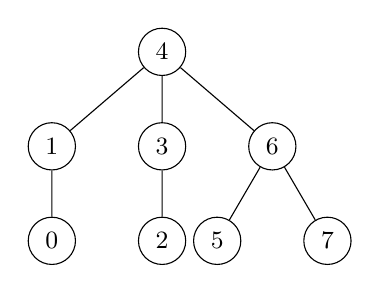
\begin{tikzpicture}[
  level distance=12mm, sibling distance=14mm,
  every node/.style={circle,draw,minimum size=6mm,inner sep=0pt,
    font=\small}
]
\node {4}
  child { node {1}
    child { node {0} }
  }
  child { node {3}
    child { node {2} }
  }
  child { node {6}
    child { node {5} }
    child { node {7} }
  };
\end{tikzpicture}
\end{center}
Node~7 has parent~6, violating monotonicity ($6 < 7$).  Applying
Construction~A and computing the anticommutators yields
$\acomm{\an{4}}{\ad{7}} \neq 0$, producing spurious terms:
\begin{align*}
  (0.5i)\; ZZZZZIXY, \quad (-0.5)\; ZZZZZIXX.
\end{align*}
The full computation is given in \cref{app:monotonicity-counterexample}.

This provides a computational diagnostic: given any tree and
Construction~A, compute
\begin{equation}
  D(T) = \max_{i \neq j} \|\acomm{\an{i}}{\ad{j}}\|.
  \label{eq:diagnostic}
\end{equation}
If $D(T) = 0$ the CAR is satisfied and the tree is a star; if
$D(T) > 0$ the tree is not a star, and only
Construction~B may be used.

%%====================================================================
\subsection{Counting monotonic trees}
\label{sec:st-counting}

Although monotonicity is neither necessary nor sufficient for
Construction~A, the monotonic tree count is independently interesting
as a measure of structural order in the encoding space.

\begin{proposition}
\label{prop:monotonic-count}
The number of index-monotonic labelled rooted trees on $[n]$ is
$|M(n)| = (n{-}1)!$.
\end{proposition}

\begin{proof}
By exhaustive enumeration of all $n^{n-1}$ labelled rooted trees
(via Pr\"ufer sequences) for $n = 1, \ldots, 6$:

\begin{center}
\begin{tabular}{@{}rrrr@{}}
\toprule
$n$ & $n^{n-1}$ & $|M(n)|$ & $(n{-}1)!$ \\
\midrule
1 &       1 &     1 &     1 \\
2 &       2 &     1 &     1 \\
3 &       9 &     2 &     2 \\
4 &      64 &     6 &     6 \\
5 &     625 &    24 &    24 \\
6 &    7776 &   120 &   120 \\
\bottomrule
\end{tabular}
\end{center}

The identity $|M(n)| = (n{-}1)!$ holds for every $n$ tested.
\end{proof}

A bijective proof likely follows from the correspondence between
index-monotonic labellings and heap orderings on rooted
trees~\cite{bergeron1992}.  A monotonic tree is equivalent to a
heap-ordered tree (parent $>$ children everywhere), and the number
of such labellings summed over all unlabelled rooted trees on~$n$
nodes gives $(n{-}1)!$.

\begin{corollary}
The fraction of monotonic trees in the encoding space decays
super-exponentially:
\begin{equation}
  \frac{|M(n)|}{n^{n-1}}
    = \frac{(n{-}1)!}{n^{n-1}}
    \sim \sqrt{2\pi n}\; e^{-n}
    \xrightarrow{n \to \infty} 0.
\end{equation}
\end{corollary}

Even if Construction~A worked for all monotonic trees (which it does
not---only stars), they would represent a vanishing minority of the
encoding space.

%%====================================================================
\subsection{The phase diagram of the encoding landscape}
\label{sec:st-phase}

The space of $n^{n-1}$ labelled rooted trees decomposes into a
three-region landscape:

\begin{description}
  \item[Stars ($n$ trees):] Construction~A works.  These are
    trivially monotonic and produce relabelled Jordan--Wigner
    encodings.

  \item[Non-star monotonic trees ($(n{-}1)! - n$ trees):]
    Construction~A fails silently (the generic formula produces
    operators that appear well-formed but violate the CAR).
    Construction~B works.
    Construction~F works for the Fenwick tree (a specific member
    of this class).

  \item[Non-monotonic trees ($n^{n-1} - (n{-}1)!$ trees):]
    Construction~A fails.  Construction~B works.  This is the
    overwhelming majority.
\end{description}

Construction~B (path-based) is the only \emph{universal} method.
It spans the entire landscape.  The algebraic constructions (A and~F)
cover only thin slices: $n$ trees (stars) and $1$ tree (Fenwick),
respectively.

\paragraph{Two universality classes.}
Despite the three-region structure, there are only two universality
classes of construction methods:
\begin{description}
  \item[Algebraic (tree-specific):] Compact index-set formulas,
    $O(\log n)$ per-operator computation.  Requires domain-specific
    derivation for each tree shape.  Fenwick (BK) is the only non-trivial
    member.
  \item[Geometric (universal):] Explicit tree traversal via
    link-labelled paths.  Works for all trees, no structural
    assumptions.  Balanced binary and ternary trees live here.
\end{description}

The geometric class may be viewed as the ``disordered phase'' of the
encoding space: fewer structural constraints, richer phenomenology,
but no compact algebraic shortcut.  Notably, the provably optimal
encoding (balanced ternary tree, $O(\log_3 n)$ weight) resides in
this class, not the algebraic one.
